\documentclass[10pt,a4paper]{article}
\usepackage[T1]{fontenc}
\usepackage[utf8]{inputenc}
\usepackage{enumitem}
\usepackage{graphicx}
\usepackage{tabularx}
\usepackage{ltablex}
\usepackage{multirow}
\usepackage{helvet}
\usepackage{hhline}
\usepackage{verbatim}
\usepackage{keystroke}
\usepackage[hidelinks]{hyperref}
\usepackage[a4paper,margin=1in]{geometry}
\usepackage{float}
\usepackage[polish]{babel}

\renewcommand\familydefault{\sfdefault}

\begin{document}
\begin{titlepage}
	\centering
	{\Large Wydział Matematyki i Nauk Informacyjnych Politechniki Warszawskiej \par}
	\vspace{1cm}
	
\includegraphics[width=0.2\textwidth]{Resources/Images/logo.png} \par
	\vspace{5cm}
	{\LARGE Wizualizacja 3D w czasie rzeczywistym\\jazdy samochodem po torze \par}
	\vspace{0.5cm}
	{\Large Tymon Felski \par}
	\vspace{1.5cm}
	{\Large Wersja 1.0.3 \par}
	\vspace{1.5cm}
	{\Large \today \par}
\end{titlepage}

\noindent
Lista zmian w dokumencie:
\begin{table}[H]
	\def\arraystretch{1.5}
	\begin{tabularx}{\textwidth}{|l|l|X|l|}
		\hline
		\textbf{Data} & \textbf{Autor} & \textbf{Opis zmian} & \textbf{Wersja} \\
		\hline
		15.12.2016 & Tymon Felski & Przygotowanie szablonu dokumentacji oraz określenie wymagań projektu & 1.0.0 \\
		\hline
		16.12.2016 & Tymon Felski & Wyznaczenie harmonogramu prac oraz architektury rozwiązania & 1.0.1 \\
		\hline
		17.01.2017 & Tymon Felski & Aktualizacja przypadków użycia aplikacji & 1.0.2 \\
		\hline
		18.01.2017 & Tymon Felski & Dodanie dokumentacji powykonawczej & 1.0.3 \\
		\hline
	\end{tabularx}
\end{table}

\newpage
\tableofcontents

\newpage
\section{Specyfikacja}

\subsection{Opis biznesowy}
Opisywany program ma za zadanie symulować jazdę samochodem po torze wyścigowym i wyświetlać użytkownikowi jej trójwymiarową wizualizację w czasie rzeczywistym.\\[\baselineskip]
Jednym z celów aplikacji jest pokazanie różnic w wyświetlaniu trójwymiarowych obiektów na ekranie w zależności od przyjętego modelu oświetlenia i trybu cieniowania. Użytkownik może wybrać jeden z dwóch dostępnych modeli oświetlenia:
\begin{enumerate}
	\item model Phonga
	\item model Blinna-Phonga
\end{enumerate}
Do wyboru dostępne są również trzy tryby cieniowania:
\begin{enumerate}
	\item cieniowanie płaskie
	\item cieniowanie Gouraud
	\item cieniowanie Phonga
\end{enumerate}
Zmiana którejkolwiek z powyższych opcji pociąga za sobą momentalną zmianę renderowanej sceny. W celu umożliwienia użytkownikowi obejrzenia widocznej sceny z wielu perspektyw, do wyboru są trzy różne ustawienia kamery:
\begin{enumerate}
	\item umiejscowiona za jadącym samochodem
	\item umiejscowiona nad torem
	\item umiejscowiona nad torem śledząca samochód
\end{enumerate}
Kamera związana z jadącym samochodem została stworzona w ten sposób, aby sprawiała wrażenie posiadania bezwładności. Podczas skręcania kamera obserwuje samochód pod kątem i wraca do położenia bezpośrednio za nim po zakończeniu skręcania. Jedną z opcji jest również wychylenie tej kamery w lewo lub prawo przy pomocy odpowiednich klawiszy.\\[\baselineskip]
Program umożliwia także rywalizację z komputerem. Użytkownik jeździ po torze razem z innym samochodem sterowanym przez komputer. Samochody są wykonane z innych materiałów, aby przedstawić różne efekty padania światła. Celem projektu nie jest realistyczne odwzorowanie kolizji pojazdów, więc interakcja modeli wpływająca na ich kształt oraz kierunek ruchu nie została zaimplementowana (modele przez siebie przenikają).\\[\baselineskip]
Do dyspozycji będą również rzeczy takie jak wiele różnobarwnych źródeł światła, drzewa, budynki i tunel ustawiony na torze w celu przetestowania świateł w samochodzie.

\newpage
\subsection{Wymagania funkcjonalne}

\subsubsection{Przypadki użycia}
Poniższy diagram UML przedstawia zbiór przypadków użycia aplikacji dla aktora -- użytkownika aplikacji.
\begin{figure}[H]
	\centering
	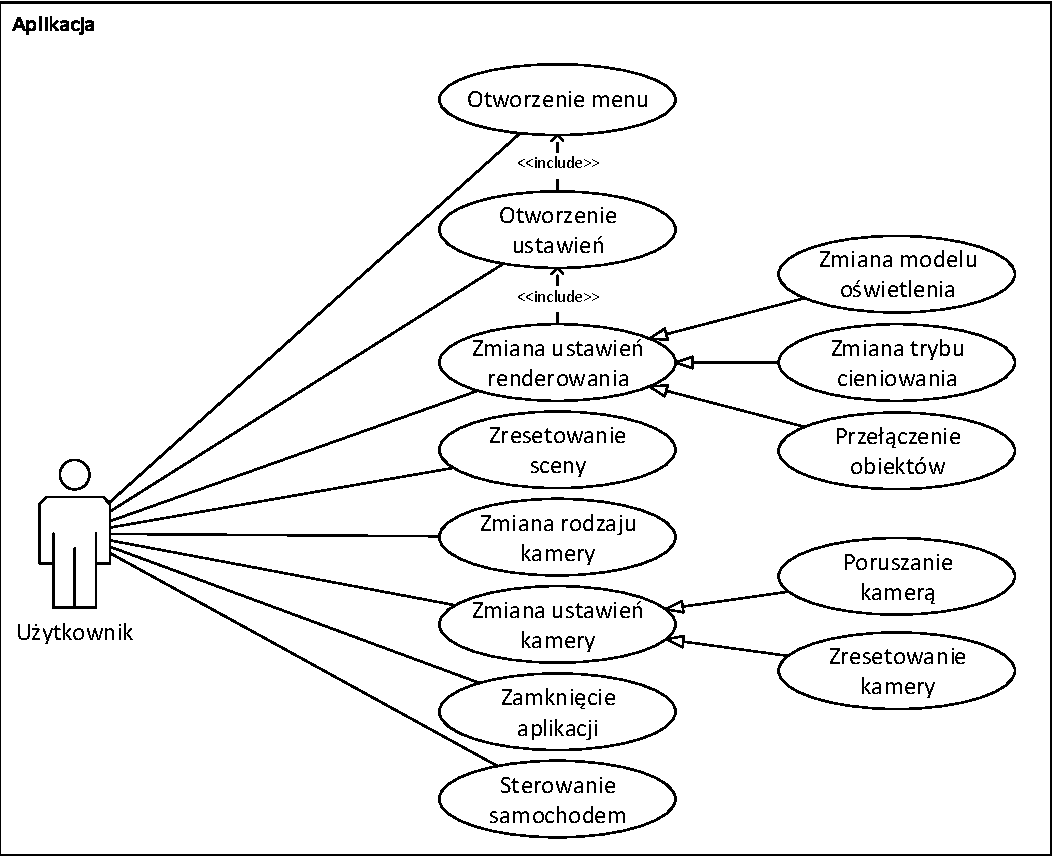
\includegraphics[width=9cm]{Resources/PDF/use-cases.pdf}
	\caption{Diagram przypadków użycia dla aplikacji}
\end{figure}

\noindent
Poszczególne przypadki są opisane szerzej w poniższej tabeli:
\begin{table}[H]
	\begin{tabularx}{\textwidth}{|c|X|X|X|}
		\hline
		\textbf{Aktor} & \textbf{Nazwa} & \textbf{Opis} & \textbf{Odpowiedź aplikacji} \\
		\hline
		\multirow{26}{*}{\rotatebox[origin=c]{90}{Użytkownik}}
		& \multirow{2}{*}{Sterowanie samochodem}
		& Wciśnięcie klawiszy \keystroke{W}\keystroke{S}\keystroke{A}\keystroke{D} na klawiaturze
		& Zmiana kierunku jazdy samochodu\\
		\cline{2-4}
		& \multirow{2}{*}{Otworzenie menu}
		& Wciśnięcie klawisza \keystroke{Esc} na klawiaturze
		& Wstrzymanie (pauza) aplikacji i wyświetlenie menu \\
		\cline{2-4}
		& \multirow{2}{*}{Otworzenie ustawień}
		& Wybranie opcji \textbf{Settings} w menu aplikacji
		& Wyświetlenie okna opcji programu \\
		\cline{2-4}
		& \multirow{3}{*}{Zmiana modelu oświetlenia}
		& \multirow{3}{*}{\parbox{4.4cm}{Wybór modelu oświetlenia w oknie ustawień programu}}
		& Wybrany model oświetlenia będzie od tego momentu używany przy renderowaniu \\
		\cline{2-4}
		& \multirow{3}{*}{Zmiana trybu cieniowania}
		& \multirow{3}{*}{\parbox{4.4cm}{Wybór trybu cieniowania w oknie ustawień programu}}
		& Wybrany tryb cieniowania będzie od tego momentu używany przy renderowaniu \\
		\cline{2-4}
		& \multirow{3}{*}{Przełączenie obiektów}
		& Wybór opcji rysowania statycznych obiektów w oknie ustawień programu
		& Włączenie lub wyłączenie rysowania statycznych obiektów na scenie \\
		\cline{2-4}
		& \multirow{2}{*}{Zresetowanie sceny}
		& Wybranie opcji \textbf{Reset} w menu aplikacji
		& Przywrócenie początkowego układu sceny \\
		\cline{2-4}
		& \multirow{2}{*}{Zmiana rodzaju kamery}
		& Wciśnięcie klawisza \keystroke{C} na klawiaturze
		& Zmiana perspektywy widocznej sceny \\
		\cline{2-4}
		& \multirow{3}{*}{Poruszanie kamerą}
		& \multirow{3}{*}{\parbox{4.4cm}{Wciśnięcie strzałek lub klawiszy \keystroke{Q}\keystroke{E} na klawiaturze}}
		& Zmiana położenia kamery statycznej lub wychylenie kamery śledzącej samochód \\
		\cline{2-4}
		& \multirow{2}{*}{Zresetowanie kamery}
		& \multirow{2}{*}{\parbox{4.4cm}{Wciśnięcie klawisza \keystroke{R} na klawiaturze}}
		& Przywrócenie początkowych ustawień obecnej kamery \\
		\cline{2-4}
		& \multirow{2}{*}{Zamknięcie aplikacji}
		& Wybranie opcji \textbf{Exit Game} w menu aplikacji
		& \multirow{2}{*}{\parbox{4.4cm}{Zamknięcie programu}} \\
		\hline
	\end{tabularx}
	\caption{Opisy przypadków użycia dla użytkownika}
\end{table}

\subsubsection{User stories}
Interfejs użytkownika:
\begin{enumerate}[label*=\arabic*.]
	\itemsep0em 
	\item \textbf{Steruję samochodem} \\
	Użytkownik ma możliwość sterowania samochodem przy użyciu klawiszy \keystroke{W}\keystroke{S}\keystroke{A}\keystroke{D}.
	\item \textbf{Otwieram główne menu aplikacji} \\
	Użytkownik może wstrzymać (zapauzować) aplikację i wyświetlić główne menu wciskając klawisz \keystroke{Esc} na klawiaturze.
	\item \textbf{Otwieram okno ustawień programu} \\
	Użytkownik jest w stanie wyświetlić okno ustwanień, wybierając opcję \textbf{Settings} w menu głównym.
	\item \textbf{Zmieniam model oświetlenia} \\
	Użytkownik ma możliwość zmiany modelu oświetlenia wykorzystywanego przy renderowaniu wizualizacji. Należy wybrać jeden jeden z dostępnych w oknie ustawień programu.
	\item \textbf{Zmieniam tryb cieniowania} \\
	Użytkownik ma możliwość zmiany trybu cieniowania wykorzystywanego przy renderowaniu wizualizacji. Należy wybrać jeden jeden z dostępnych w oknie ustawień programu.
	\item \textbf{Przełączam obiekty} \\
	Użytkownik może włączyć lub wyłączyć rysowanie obiektów statycznych na scenie. Należy zaznaczyć lub odznaczyć checkbox w oknie ustawień programu.
	\item \textbf{Resetuję scenę} \\
	Użytkownik jest w stanie przywrócić układ sceny do stanu początkowego, wybierając opcję \textbf{Reset} w menu głównym.
	\item \textbf{Zmieniam rodzaj kamery} \\
	Użytkownik może zmienić kamerę, z której oglądana jest scena. Wciśnięcie klawisza \keystroke{C} spowoduje przewinięcie do kolejnej kamery w sekwencji dostępnych.
	\item \textbf{Poruszam kamerą} \\
	Użytkownik ma możliwość zmiany położenia kamery statycznej strzałkami lub wychylenia kamery umiejscowionej za samochodem klawiszami \keystroke{Q}\keystroke{E}.
	\item \textbf{Resetuję kamerę} \\
	Użytkownik może przywrócić początkowe ustawienia kamery, wciskając klawisz \keystroke{R}.
	\item \textbf{Zamykam aplikację} \\
	Użytkownik jest w stanie wyjść z programu, wybierając opcję \textbf{Exit Game} w menu głównym.
\end{enumerate}

\subsection{Wymagania niefunkcjonalne}
Poniższa tabela zawiera rozpisane wymagania niefunkcjonalne narzucone dla aplikacji.
\begin{table}[H]
	\begin{tabularx}{\textwidth}{|c|c|X|}
		\hline
		\textbf{Obszar wymagań} & \textbf{Nr} & \textbf{Opis} \\
		\hline
		\multirow{3}{*}{Użyteczność (\textit{Usability})}
		& 1
		& Interfejs użytkownika powinien być w języku angielskim. \\
		\cline{2-3}
		& \multirow{2}{*}{2}
		& Interfejs użytkownika powinnien być w pełni wspierany i dostępny w okienku o rozdzielczości 1280x720. \\
		\hline
		\multirow{2}{*}{Niezawodność (\textit{Reliability})}
		& \multirow{2}{*}{3}
		& Aplikacja musi być w stanie obsłużyć możliwe błędy i nie dopuścić do ich wyświetlania na ekranie w formie artefaktów. \\
		\hline
		\multirow{5}{*}{Wydajność (\textit{Performance})}
		& \multirow{2}{*}{4}
		& Aplikacja powinna generować wizualizację w przynajmniej 10 klatkach na sekundę. \\
		\cline{2-3}
		& 5
		& Zużycie pamięci RAM nie powinno przekroczyć 500MB. \\
		\cline{2-3}
		& \multirow{2}{*}{6}
		& Czas odpowiedzi aplikacji na polecenie użytkownika powinień być nie dłuższy niż 200ms. \\
		\hline
		\multirow{4}{*}{Utrzymanie (\textit{Supportability})}
		& \multirow{2}{*}{7}
		& Uruchomienie aplikacji powinno być możliwe na systemach Windows 7 i nowszych. \\
		\cline{2-3}
		& \multirow{2}{*}{8}
		& Aplikacja powinna wspierać karty graficzne AMD Radeon HD7870 oraz NVIDIA GeForce GTX660M i nowsze. \\
		\hline
	\end{tabularx}
	\caption{Tabela wymagań niefunkcjonalnych}
\end{table}

\newpage
\subsection{Harmonogram projektu}
Prace przy projekcie będą realizowane według następującego harmonogramu:
\begin{figure}[H]
	\centering
	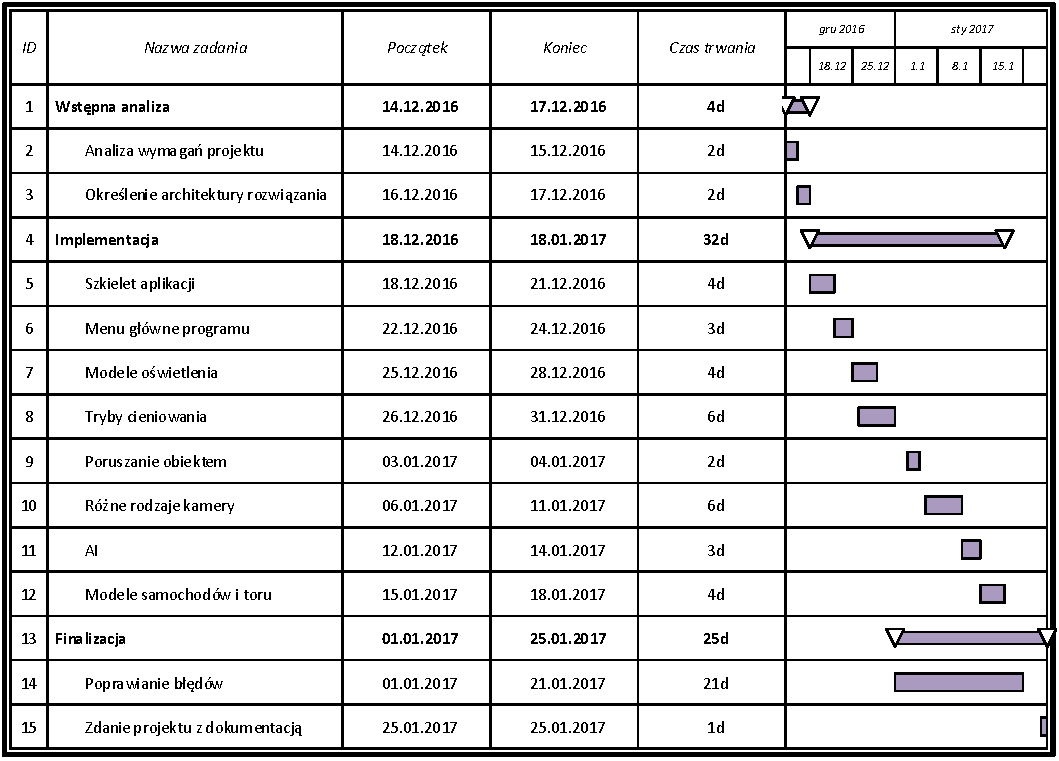
\includegraphics[width=16cm]{Resources/PDF/gantt.pdf}
	\caption{Diagram Gantta z planowanym harmonogramem projektu}
\end{figure}

\noindent
Kamienie milowe:
\begin{enumerate}
	\item \textbf{14 grudnia:} Rozpoczęcie prac nad specyfikacją wstępną. Analiza wymagań projektu.
	\item \textbf{17 grudnia:} Określenie architektury rozwiązania. Zakończenie dokumentacji wstępnej.
	\item \textbf{21 grudnia:} Utworzenie wstępnego szkieletu aplikacji umożliwiającego renderowanie sceny.
	\item \textbf{24 grudnia:} Dodanie głównego menu programu.
	\item \textbf{28 grudnia:} Zaimplementowanie modeli oświetlenia.
	\item \textbf{31 grudnia:} Zaimplementowanie trybów cieniowania.
	\item \textbf{4 stycznia:} Dodanie możliwości poruszania obiektem.
	\item \textbf{11 stycznia:} Implementacja różnych rodzajów kamery.
	\item \textbf{14 stycznia:} Dodanie obiektów sterowanych przez komputer.
	\item \textbf{18 stycznia:} Dodanie modeli samochodów i toru.
	\item \textbf{21 stycznia:} Zakończenie poprawiania błędów.
	\item \textbf{25 stycznia:} Zdanie projektu łącznie z pełną dokumentacją.
\end{enumerate}

\newpage
\subsection{Architektura rozwiązania}
Poniższy diagram UML przedstawia schemat architektury aplikacji.
\begin{figure}[H]
	\centering
	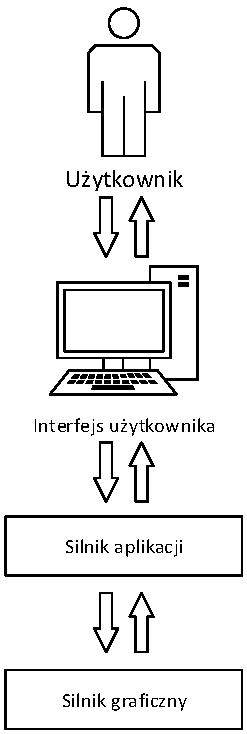
\includegraphics[width=4cm]{Resources/PDF/system-architecture.pdf}
	\caption{Diagram architektury aplikacji}
\end{figure}

\noindent
Użytkownik korzysta z aplikacji przy pomocy graficznego interfejsu. Wydaje za jego pomocą polecenia, które bezpośrednio wpływają na wygląd renderowanej sceny. Polecenia są interpretowane i przetwarzane przez silnik aplikacyjny, który po wykonaniu odpowiednich obliczeń, wykorzystuje silnik graficzny, aby wyświetlić scenę na ekranie.\\[\baselineskip]
Silnikiem graficznym użytym w projekcie jest framework XNA. Jest to biblioteka wydana przez firmę Microsoft, pozwalająca na tworzenie gier przeznaczonych dla systemu Windows, konsoli Xbox 360 jak również telefonów z systemem operacyjnym Windows Phone. Umożliwia ona osiągnięcie dobrej wydajności oraz łatwe wsparcie interakcji z użytkownikiem, na przykład poprzez obsługę wibracji w kontrolerach.

\newpage
\section{Dokumentacja końcowa (powykonawcza)}

\subsection{Wymagania systemowe}
Aby zapewnić poprawne działanie aplikacji, wymagane są następujące komponenty:
\begin{enumerate}
	\item Windows 7 lub nowszy.
	\item Minimum 512MB pamięci RAM.
	\item Karta graficzna AMD Radeon HD7870 lub NVIDIA GeForce GTX660M lub nowsze.
\end{enumerate}

\subsection{Biblioteki wraz z określeniem licencji}
Przy tworzeniu projektu zostały użyte następujące biblioteki:

\begin{table}[H]
	\begin{tabularx}{\textwidth}{|r|l|X|l|c|}
		\hline
		\textbf{Nr} & \textbf{Komponent i wersja} & \textbf{Opis} & \textbf{Licencja} & \\
		\hline
		1 & 
		Microsoft XNA Game Studio, 4.0.5 &
		Framework pozwalający na tworzenie gier dla systemu Windows. &
		\mbox{\hyperref[abbr:eula]{EULA}} &
		\cite{xna} \\
		\hline
		2 &
		NeoForce Controls, 2.1 &
		Zbiór kontrolek UI przeznaczonych do aplikacji XNA. &
		\mbox{\hyperref[abbr:lgpl]{LGPL}} &
		\cite{neoforce} \\
		\hline
	\end{tabularx}
	\caption{Lista użytych bibliotek}
\end{table}

\subsection{Instrukcja instalacji}
Aby zainstalować aplikację należy wykonać następujące kroki:
\begin{enumerate}
	\item Rozpakować archiwum \textbf{ProjectCars.zip} z plikami gry.
	\item Przenieść/skopiować katalog z plikami gry do folderu docelowego.
\end{enumerate}

\subsection{Instrukcja uruchomienia}
W celu uruchomienia programu, klikamy dwukrotnie plik wykonywalny \textbf{ProjectCars.exe}.

\newpage
\subsection{Instrukcja użycia}
Scena jest gotowa od razu po uruchomieniu aplikacji -- nie jest wymagana wcześniejsza konfiguracja.

\subsubsection{Jazda samochodem}
Aby wykonać ruch samochodem, należy wcisnąć jeden z klawiszy \keystroke{W}\keystroke{S}\keystroke{A}\keystroke{D}, które odpowiadają odpowiednio jeździe do przodu i do tyłu oraz skręcaniu w lewo i prawo.

\subsubsection{Przełączenie świateł samochodów}
Przy pomocy klawisza \keystroke{L} można włączyć lub wyłączyć reflektory w samochodach.
\begin{figure}[H]
  \centering
  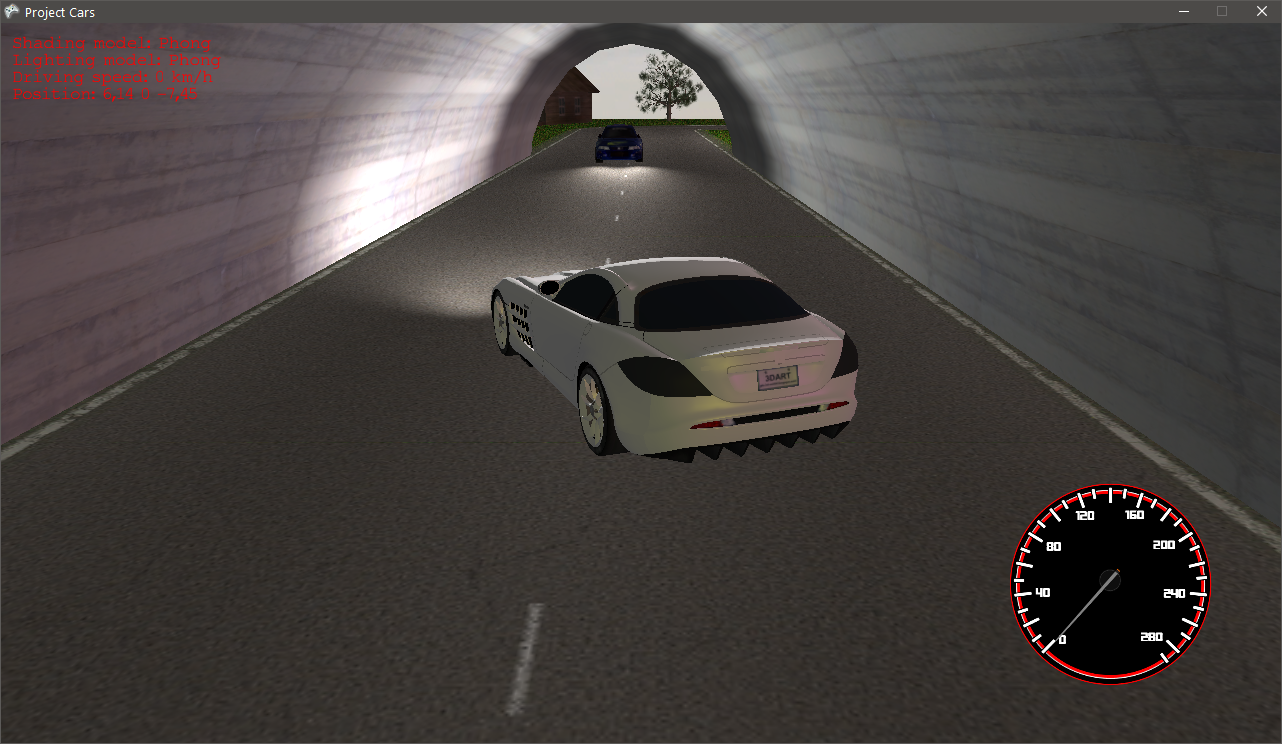
\includegraphics[width=11cm]{Resources/Images/tunnel.png}
  \caption{Reflektory samochodów widoczne w tunelu}
\end{figure}

\subsubsection{Resetowanie sceny}
Aby przywrócić scenę do konfiguracji początkowej, należy wybrać opcję \textbf{Reset} w menu głównym.

\subsubsection{Zmiana rodzaju kamery}
W programie przygotowano zestaw trzech kamer, pomiędzy którymi można przełączać się przy pomocy klawisza \keystroke{C}. Zmiana jest cykliczna, więc po osiągnięciu ostatniej, nastąpi przełączenie do pierwszej. Domyślna kamera jest umiejscowiona za samochodem.
\begin{figure}[H]
  \centering
  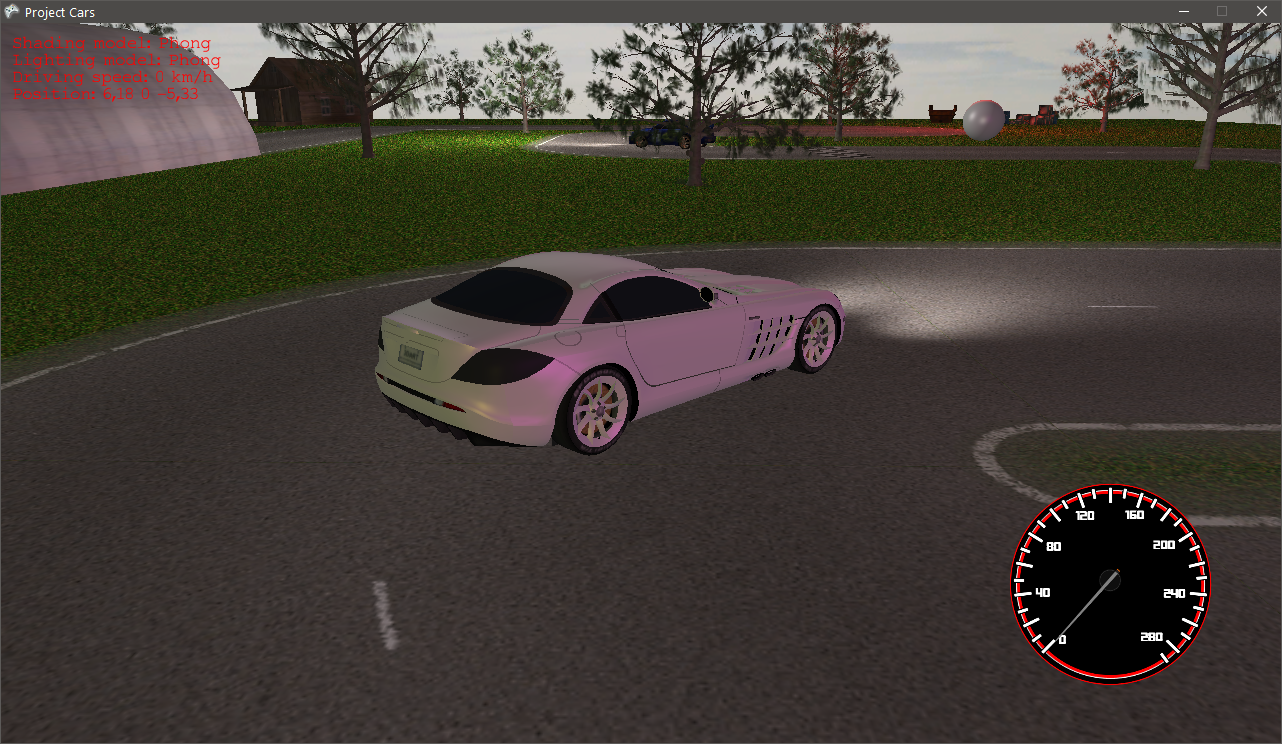
\includegraphics[width=11cm]{Resources/Images/cam_car.png}
  \caption{Kamera umiejscowiona za samochodem}
\end{figure}
\begin{figure}[H]
  \centering
  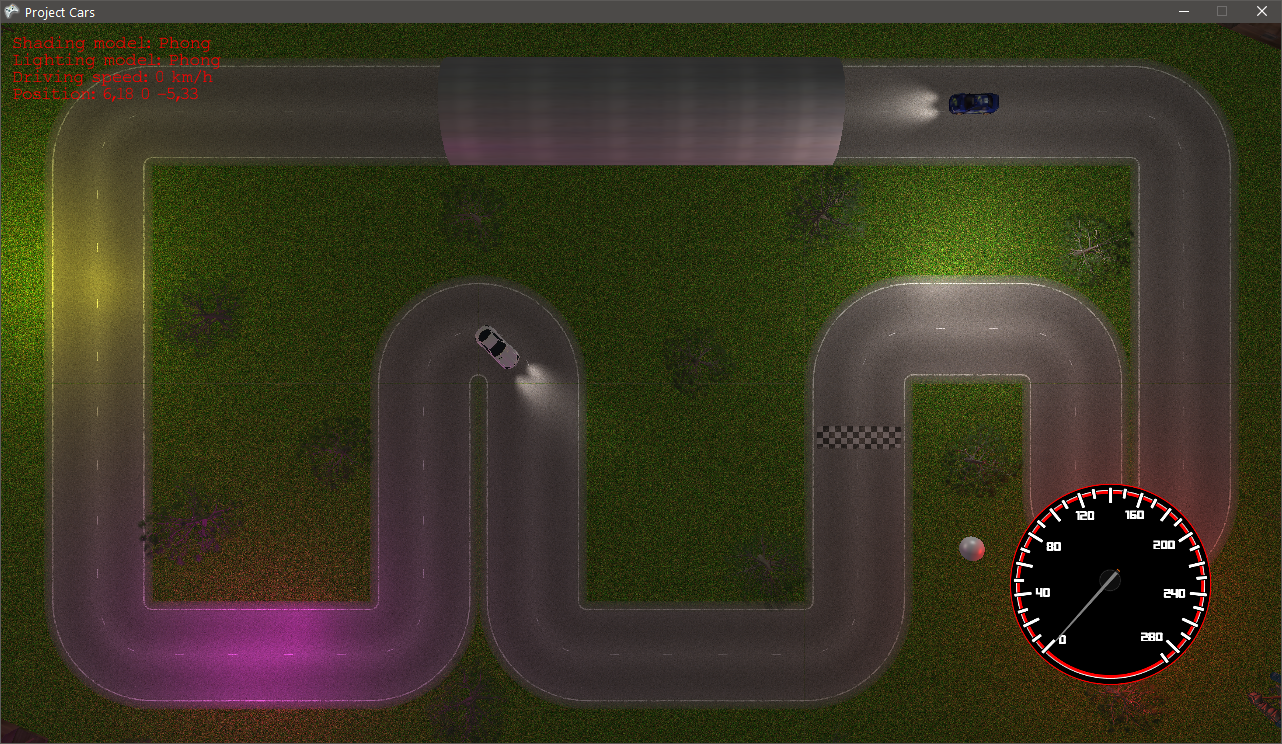
\includegraphics[width=11cm]{Resources/Images/cam_static.png}
  \caption{Kamera statyczna}
\end{figure}
\begin{figure}[H]
  \centering
  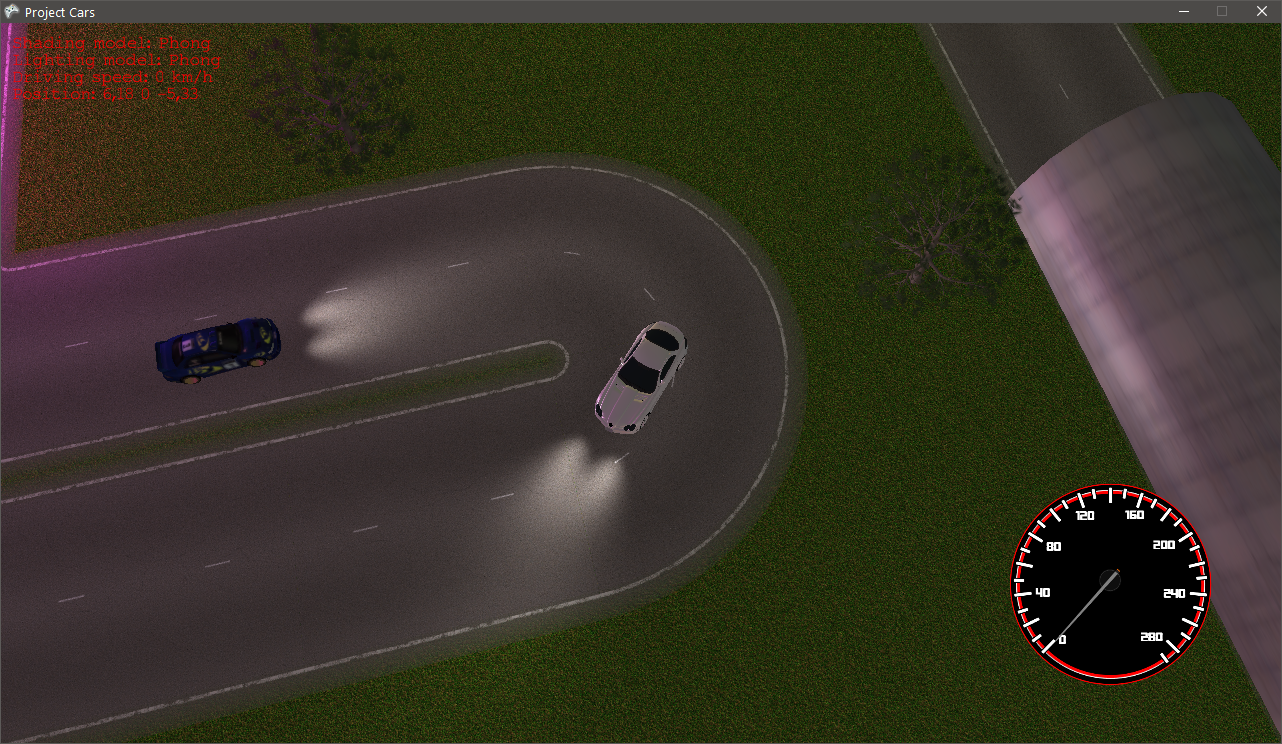
\includegraphics[width=11cm]{Resources/Images/cam_follow.png}
  \caption{Kamera śledząca}
\end{figure}

\subsubsection{Zmiana położenia kamery}
Kamera umiejscowiona za samochodem może zostać obrócona w lewo lub prawo przy pomocy klawiszy \keystroke{Q}\keystroke{E}. Kamery statyczne można przesuwać przy pomocy strzałek. Wciśnięcie klawisza \keystroke{R} spowoduje przywrócenie ustawień początkowych obecnie wybranej kamery.

\newpage
\subsubsection{Otworzenie menu głównego}
Po wciśnięciu klawisza \keystroke{Esc}, gra zostanie wstrzymana (zapauzowana), a następnie wyświetli się główne menu aplikacji.
\begin{figure}[H]
  \centering
  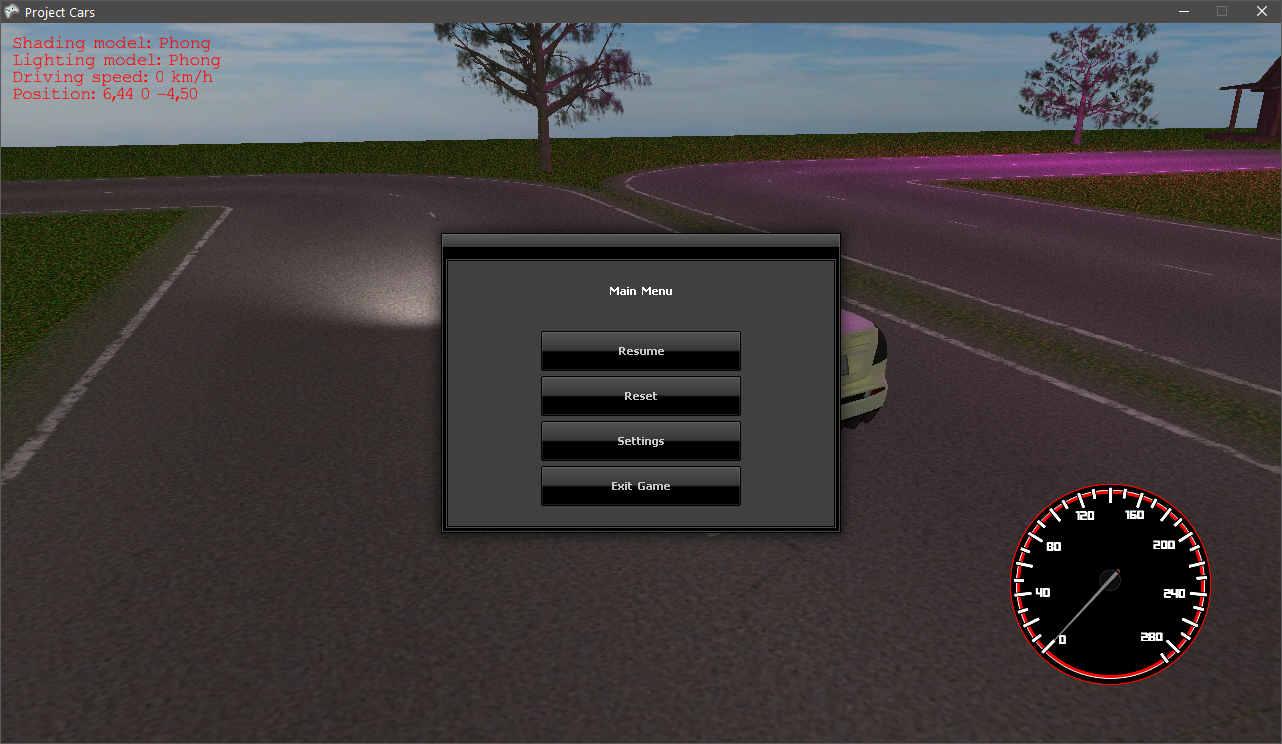
\includegraphics[width=11cm]{Resources/Images/menu_main.png}
  \caption{Menu główne aplikacji}
\end{figure}

\subsubsection{Zmiana modelu oświetlenia i trybu cieniowania}
Wchodzimy do okna ustawień programu, wybierając opcję \textbf{Settings} w menu głównym. Znajdują się tam dwa comboboxy podpisane odpowiednio \textbf{Shading model} oraz \textbf{Lighting model} służące do wyboru trybu cieniowania i modelu oświetlenia używanego przy renderowaniu. Wybranie któregokolwiek z nich będzie skutkować natychmiastową zmianą w rysowaniu sceny.
\begin{figure}[H]
  \centering
  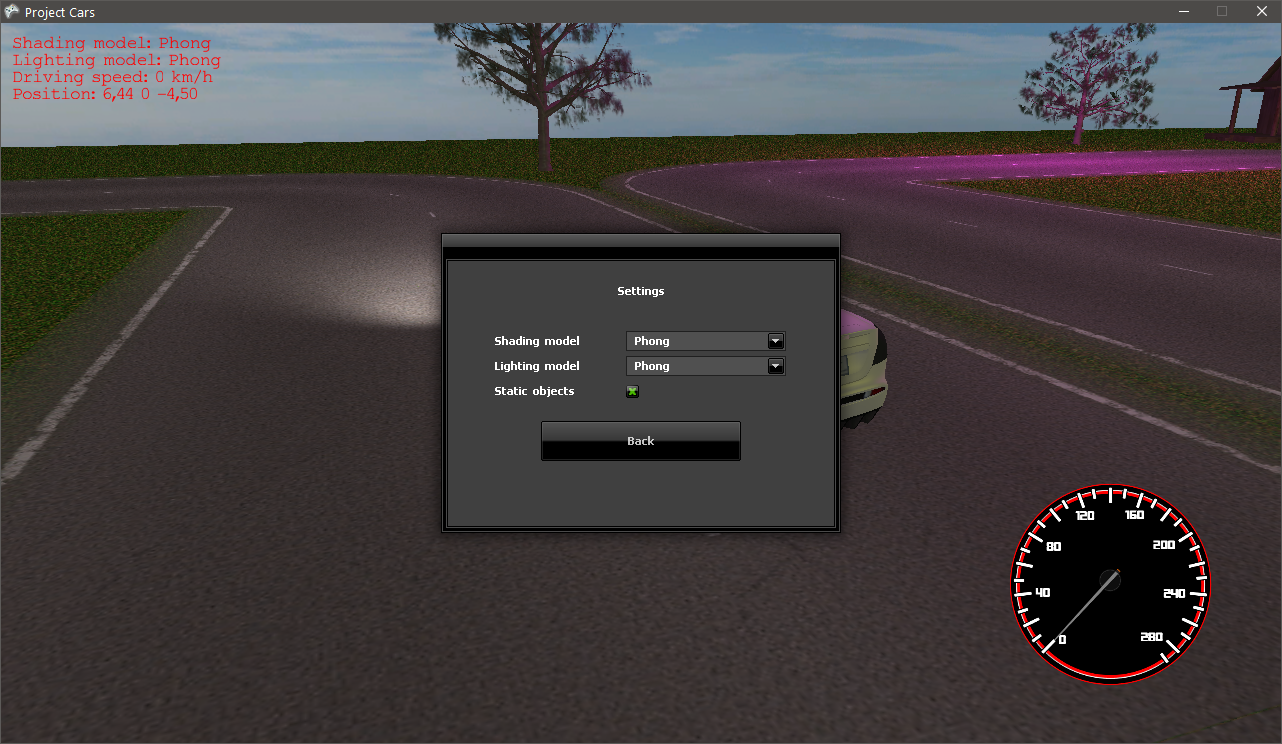
\includegraphics[width=11cm]{Resources/Images/menu_settings.png}
  \caption{Okno ustawień programu}
\end{figure}

\subsubsection{Przełączanie obiektów na scenie}
W oknie ustawień programu znajduje się checkbox podpisany \textbf{Static objects}, którego zaznaczenie lub odznaczenie spowoduje odpowiednio pokazanie lub ukrycie statycznych obiektów znajdujących się na scenie.

\subsubsection{Zamknięcie aplikacji}
Wyjście z gry jest możliwe poprzez wybranie opcji \textbf{Exit Game} w menu głównym.

\subsection{Raport odstępstw od specyfikacji wymagań}
Brak.

\section{Dokumentacja końcowa (powykonawcza) -- punkty wymagane przez prowadzącego zajęcia}

\subsection{Scenariusze testów akceptacyjnych i raport z ich przeprowadzenia}

\begin{tabularx}{\textwidth}{|l|X|}
	\hline
	\textbf{Nazwa testu} & Poruszanie samochodem \\
	\hline
	\textbf{Opis} & Wciśnięcie klawiszy \keystroke{W}\keystroke{S}\keystroke{A}\keystroke{D} na klawiaturze w czasie działania programu. \\
	\hline
	\textbf{Oczekiwany wynik} & Jazda samochodem do przodu i do tyłu z możliwością skręcania. \\
	\hline
	\textbf{Wynik testu} & Pozytywny \\
	\hhline{==}
	\textbf{Nazwa testu} & Zmiana rodzaju kamery \\
	\hline
	\textbf{Opis} & Wciśnięcie przycisku \keystroke{C} na klawiaturze podczas działania aplikacji. \\
	\hline
	\textbf{Oczekiwany wynik} & Cykliczna zmiana kamery używanej do obserwowania sceny. \\
	\hline
	\textbf{Wynik testu} & Pozytywny \\
	\hhline{==}
	\textbf{Nazwa testu} & Poruszanie kamerą i przywracanie położenia początkowego \\
	\hline
	\textbf{Opis} & Wciśnięcie przycisków \keystroke{Q}\keystroke{E} przy kamerze umiejscowionej za samochodem lub strzałek przy kamerze statycznej. Wciśnięcie klawisza \keystroke{R}, aby zresetować ustawienia obecnej kamery. \\
	\hline
	\textbf{Oczekiwany wynik} & Wychylenie kamery umiejscowionej na samochodem, zmiana położenia kamer statycznych oraz przywrócenie położenia początkowego danej kamery. \\
	\hline
	\textbf{Wynik testu} & Pozytywny \\
	\hhline{==}
	\textbf{Nazwa testu} & Zmiana trybu cieniowania \\
	\hline
	\textbf{Opis} & Wybranie jednego z trybów cieniowania w oknie ustawień programu. \\
	\hline
	\textbf{Oczekiwany wynik} & Natychmiastowa zmiana obrazu wyświetlanego na ekranie oraz tekstu w lewym górnym rogu ekranu. \\
	\hline
	\textbf{Wynik testu} & Pozytywny \\
	\hhline{==}
	\textbf{Nazwa testu} & Zmiana modelu oświetlenia \\
	\hline
	\textbf{Opis} & Wybranie jednego z modeli oświetlenia w oknie ustawień programu. \\
	\hline
	\textbf{Oczekiwany wynik} & Natychmiastowa zmiana obrazu wyświetlanego na ekranie oraz tekstu w lewym górnym rogu ekranu. \\
	\hline
	\textbf{Wynik testu} & Pozytywny \\
	\hhline{==}
	\textbf{Nazwa testu} & Włączenie/wyłączenie obiektów statycznych na scenie lub świateł w samochodach \\
	\hline
	\textbf{Opis} & Zaznaczenie/odznaczenie checkboxa \textbf{Static objects} w oknie ustawień programu. Wciśnięcie klawisza \keystroke{L} w celu przełączenia reflektorów. \\
	\hline
	\textbf{Oczekiwany wynik} & Przełączenie obiektów statycznych na scenie i świateł w samochodach. \\
	\hline
	\textbf{Wynik testu} & Pozytywny \\
	\hhline{==}
	\textbf{Nazwa testu} & Zresetowanie sceny \\
	\hline
	\textbf{Opis} & Wybranie opcji \textbf{Reset} w menu głównym aplikacji. \\
	\hline
	\textbf{Oczekiwany wynik} & Przywrócenie konfiguracji początkowej wyświetlanej sceny. \\
	\hline
	\textbf{Wynik testu} & Pozytywny \\
	\hhline{==}
	\textbf{Nazwa testu} & Zamknięcie aplikacji \\
	\hline
	\textbf{Opis} & Wybranie opcji \textbf{Exit Game} w menu głównym aplikacji. \\
	\hline
	\textbf{Oczekiwany wynik} & Wyłączenie się programu. \\
	\hline
	\textbf{Wynik testu} & Pozytywny \\
	\hline
\end{tabularx}

\newpage
\section{Lista użytych skrótów}
\label{abbr:eula}
\paragraph{EULA} End User License Agreement

\label{abbr:lgpl}
\paragraph{LGPL} GNU Library General Public License

\renewcommand*{\refname}{\vspace*{-2em}}
\section{Bibliografia}
\begin{thebibliography}{99}
	\bibitem{xna}
		XNA Game Studio,
		\emph{Microsoft},
		\url{https://www.microsoft.com/en-us/download/details.aspx?id=23714}

	\bibitem{neoforce}
		NeoForce Controls for XNA,
		\emph{Tom Shane},
		\url{https://github.com/NeoforceControls/XNA}
\end{thebibliography}

\end{document}
